% Tikz File 'mytikz.tex'
\documentclass{standalone}
%\input{../../Mod_base/grafica}
\input{../Mod_base/grafica}
\input{simboli_operatori}
\input{../Mod_base/unita_misura}
%\usetikzlibrary{...}
\begin{document}
\begin{tikzpicture}
\begin{axis}
[xmin=-6,xmax=6,ymin=-1,ymax=6, %grid,
axis x line=middle,xtick={-6,-5,...,6},ytick={-6,-5,...,6},
axis y line=middle,xlabel=$x$,ylabel=$y$]
%\addplot[samples=200] {(1^(x))};
\addplot [samples=200] {(0.83^(x))};
\addplot [samples=200] {(0.67^(x))};
\addplot [samples=200] {(0.5^(x))};
\end{axis}
%\node (a1) at (1,2) {$y=1^x$};
\node (a2) at (1,2.2) {$y=(\dfrac{5}{6})^x$};
\node (a3) at (1.1,4.2) {$y=(\dfrac{2}{3})^x$};
\node (a3) at (2.1,5) {$y=\dfrac{1}{2}^x$};
\end{tikzpicture}
\end{document}